\subsection{余结合性、余交换性、余单位}

设 E 为一个余代数，c 为其余积，N, N', N'' 为三个 A-模，m 为 N × N' 到 N'' 的一个双线性映射。设 \(\tilde{m}:N \otimes_{A} N' \to N''\) 为对应于 m 的 A-线性映射。若 \(u:E \to N\) , \(v:E \to N'\) 是两个 A-线性映射，我们得到一个 A-线性映射 \(u \otimes v:E \otimes_{A} E \to N \otimes_{A} N'\) 以及一个从 E 到 N'' 的复合 A-线性映射：

\[
m (u, v): \mathrm{E} \xrightarrow {c} \mathrm{E} \otimes_ {\mathrm{A}} \mathrm{E} \xrightarrow {u \otimes v} \mathrm{N} \otimes_ {\mathrm{A}} \mathrm{N} ^ {\prime} \xrightarrow {\tilde {m}} \mathrm{N} ^ {\prime \prime}.\tag{11}
\]

显然，我们由此定义了一个 A-双线性映射 \((u, v) \mapsto m(u, v)\) ，它从 \(\operatorname{Hom}_{\mathbf{A}}(\mathbf{E}, \mathbf{N}) \times \operatorname{Hom}_{\mathbf{A}}(\mathbf{E}, \mathbf{N}')\) 到 \(\operatorname{Hom}_{\mathbf{A}}(\mathbf{E}, \mathbf{N}'')\) 中。

当 E 为分次余代数，N, N', N'' 为同类型的分次 A-模，且 \(\tilde{m}\) 为从 N \(\otimes_{A}N'\) 到 N'' 的 k 次分次同态时，若 u（相应地 v）是 p 次（相应地 q 次）分次同态，则 \(m(u,v)\) 是次数为 \(p + q + k\) 的分次同态。

例。（1）取 E 为分次余代数 T(M)（第 1 号），并假设 N, N', N'' 具有平凡分次。则从 T(M) 到 N（相应地 N', N''）的 -p 次分次同态对应于从 M\^{}p 到 N（相应地 N', N''）的多重线性映射。给定一个多重线性映射 u: M\^{}p → N 和一个多重线性映射 v: M\^{}q → N'，上述方法使我们能够推导出一个多重线性映射 m(u, v)：M\^{}\{p+q\} → N''，称为u与v的（关于m的）乘积。公式（3）（第1号）和（11）表明，对于M中的x\_1, . . ., x\_p+q，

\[
(m (u, v)) \left(x _ {1}, \dots , x _ {p + q}\right) = m \left(u \left(x _ {1}, \dots , x _ {p}\right), v \left(x _ {p + 1}, \dots , x _ {p + q}\right)\right).
\]

\begin{enumerate}
\def\labelenumi{(\arabic{enumi})}
\setcounter{enumi}{1}
\tightlist
\item
  设 E 为分次余代数 S(M)（第 1 号），对 N、N'、N'' 保持相同的假设。从 S(M) 到 N 的 −p 次分次同态对应于从 M \(^{p}\) 到 N 的对称多重线性映射（§ 6，第 3 号）。于是，由对称多重线性映射 u: M \(^{p}\) → N 和对称多重线性映射 v: M \(^{q}\) → N' 得到一个对称多重线性映射 m(u, v)：M \(^{p+q}\) → N''，也（为避免混淆）记作 \(u \cdot_{m} v\) （甚至 \(u \cdot v\)），并称为 u 和 v 的（关于 m 的）对称积。公式 (6)（第 1 号）和 (11) 表明，对于 M 中的 x₁， \ldots， \(_{p+q}\) ，
\end{enumerate}

\[
(u \cdot_{m} v) (x _ {1}, \dots , x _ {p + q}) = \sum_ {\sigma} m (u (x _ {\sigma (1)}, \dots , x _ {\sigma (p)}), v (x _ {\sigma (p + 1)}, \dots , x _ {\sigma (p + q)}))
\]

求和遍历所有置换 \(\sigma\in\mathfrak{S}_{p+q}\) ，这些置换在每个区间 \([1,p]\) 和 \([p+1,p+q]\) 上都是递增的。

\begin{enumerate}
\def\labelenumi{(\arabic{enumi})}
\setcounter{enumi}{2}
\tightlist
\item
  取 E 为分次余代数 \(\bigwedge (\mathbf{M})\) （第 1 号）。于是我们类似地从交错多重线性映射 \(u: \mathbf{M}^p \to \mathbf{N}\) 和交错多重线性映射 \(v: \mathbf{M}^q \to \mathbf{N}'\) 得到一个交错多重线性映射 \(m(u, v): \mathbf{M}^{p + q} \to \mathbf{N}''\) ，也记作 \(u \wedge_m v\) 或 \(u \wedge v\) ，并称为（关于 \(m\) 的） \(u\) 和 \(v\) 的交错积。公式（9）（第 1 号）和（11）表明在这种情况下，对于 \(x_1, \ldots, x_{p + q}\) （在 \(\mathbf{M}\) 中），
\end{enumerate}

\[
(u \wedge_ {m} v) (x _ {1}, \dots , x _ {p + q}) = \sum_ {\sigma} \varepsilon_ {\sigma} m (u (x _ {\sigma (1)}, \dots , x _ {\sigma (p)}), v (x _ {\sigma (p + 1)}, \dots , x _ {\sigma (p + q)}))
\]

求和再次遍历所有排列 \(\sigma \in \mathfrak{S}_{p + q}\) ，这些排列在每个区间 \([1, p]\) 和 \([p + 1, p + q]\) 上都是递增的。

我们回到 E 为任意分次余代数（N 型）的情形，并假设三个模 N、N'、N'' 都等于一个 Z 型分次 A-代数 B 的底层 A-模，映射 m 为 B 中的乘法，从而 \(\tilde{m}:B\otimes_{A}B\to B\) 是一个次数为 0 的分次 A-线性映射。于是在分次 A-模 \(\operatorname{Homgr}_{A}(E,B)=C\) 上获得了一个分次 A-代数结构。

特别地，假设 B = A（具有平凡分次），因此 \(\operatorname{Homgr}_{\mathbf{A}}(\mathbf{E}, \mathbf{A})\) 是分次对偶 \(E^{*gr}\) ，从而它具有一个分次 A-代数结构。

设 F 为另一个分次余代数， \(c'\) 为其余积， \(\phi:E\to F\) 为一个分次余代数态射（第1号）；则典范分次态射

\[
\tilde {\phi} = \operatorname{Hom} (\phi , 1 _ {B}): \operatorname{Homgr} _ {A} (F, B) \rightarrow \operatorname{Homgr} _ {A} (E, B)
\]

是一个分次代数同态。对于 \(u, v\) 在 \(\operatorname{Homgr}_{\mathbf{A}}(\mathbf{F}, \mathbf{B})\) 和 \(x \in \mathbf{E}\) ,

\[
(\tilde {\phi} (u v)) (x) = (u v) (\phi (x)) = m ((u \otimes v) (c ^ {\prime} (\phi (x))))
\]

但根据假设 \(c'(\phi(x)) = (\phi \otimes \phi)(c(x))\) ，因此

\[
(u \otimes v) (c ^ {\prime} (\phi (x))) = (\tilde {\phi} (u) \otimes \tilde {\phi} (v)) (c (x))
\]

，从而 \(\tilde{\phi}(uv) = \tilde{\phi}(u)\tilde{\phi}(v)\) ，这证明了我们的断言。

特别地，分次转置 \({}^{t}\phi: \mathrm{F}^{*gr} \to \mathrm{E}^{*gr}\) 是分次代数同态。

注：假设诸 \(E_{p}\) 是有限生成的投射 A-模，因此分次 A-模（ \(E \otimes_{A} E)^{*gr}\) 和 \(E^{*gr} \otimes_{A} E^{*gr}\) 可以典范地等同（II，§4，第4号，命题4的推论1）。如果 A-模 \(A \otimes_{A} A\) 和 A 也被典范地等同（II，§3，第4号），则线性映射 \(E^{*gr} \otimes_{A} E^{*gr} \to E^{*gr}\) （它定义了 \(E^{*gr}\) 中的乘法）可称为余积 c 的分次转置。

命题1. 设 E 是 A 上的余代数。为使对每个结合 A-代数 B，A-代数 \(\operatorname{Hom}_{\mathbf{A}}(\mathbf{E}, \mathbf{B})\) 是结合的，其充分必要条件是余积 \(c: \mathbf{E} \to \mathbf{E} \otimes_{\mathbf{A}} \mathbf{E}\) 使得图表

\begin{enumerate}
\def\labelenumi{(\arabic{enumi})}
\setcounter{enumi}{11}
\tightlist
\item
\end{enumerate}

\pandocbounded{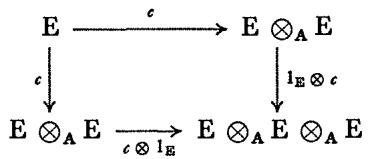
\includegraphics[keepaspectratio]{images/part004_a79ed2ff.jpg}}

是交换的。

设 B 是一个结合 A-代数，且 u、v、w 是 \(\mathbf{C} = \operatorname{Hom}_{\mathbf{A}}(\mathbf{E}, \mathbf{B})\) 的三个元素。设 \(m_{3}\) 表示 A-线性映射 \(B \otimes_{A} B \otimes_{A} B \to B\) ，它把 \(b \otimes b' \otimes b''\) 映为 \(bb'b''\) 。根据代数 C 上乘积的定义， \((uv)w\) 是复合映射

\[
\mathrm{E} \xrightarrow {c} \mathrm{E} \otimes \mathrm{E} \xrightarrow {c \otimes 1 _ {\mathrm{E}}} \mathrm{E} \otimes \mathrm{E} \otimes \mathrm{E} \xrightarrow {u \otimes v \otimes w} \mathrm{B} \otimes \mathrm{B} \otimes \mathrm{B} \xrightarrow {m _ {3}} \mathrm{B}
\]

而 \(u(vw)\) 是复合映射，

\[
\mathrm{E} \xrightarrow {c} \mathrm{E} \otimes \mathrm{E} \xrightarrow {1 _ {\mathrm{E}} \otimes c} \mathrm{E} \otimes \mathrm{E} \otimes \mathrm{E} \xrightarrow {u \otimes v \otimes w} \mathrm{B} \otimes \mathrm{B} \otimes \mathrm{B} \xrightarrow {m _ {3}} \mathrm{B}.
\]

由此可知，若图表 (12) 可交换，则代数 \(\operatorname{Hom}_{\mathbf{A}}(\mathbf{E}, \mathbf{B})\) 对每个结合的A-代数B都是结合的。为建立其逆命题，只需证明存在一个结合的A-代数B以及三个A-线性映射 \(u, v, w\) 将E映入B，使得该映射 \(m_3 \circ (u \otimes v \otimes w)\) 从 \(\mathbf{E} \otimes \mathbf{E} \otimes \mathbf{E}\) 到 B 中是单射。取 B 为 A-代数 \(\mathsf{T}(\mathbf{E})\) ， \(u, v, w\) 为 E 到 \(\mathsf{T}(\mathbf{E})\) 的典范映射。该映射 \(m_3 \circ (u \otimes v \otimes w)\) 就是典范映射 \(\mathbf{E} \otimes \mathbf{E} \otimes \mathbf{E} = \mathsf{T}^3(\mathbf{E}) \to \mathsf{T}(\mathbf{E})\) ，它是单射的。

当余代数 E 满足命题 1 的条件时，称其为余结合的。

例子。(4) 容易直接验证，余代数 A（第 1 号，例 (1)）以及余代数 \(\mathbf{A}^{(\mathbf{X})}\) （第1号，例4）和余代数 \(\mathbf{T}(\mathbf{M})\) （第1号，例5）是余结合的。若B是一个结合A-代数，且是有限生成的投射A-模，则余代数 \(\mathbf{B}^*\) （第1号，例3）是余结合的：因为此时图(12)的交换性可由表达B的结合性的图的交换性通过转置得到（ \(\S\) 1，第3号）。反之，同样的论证以及 A-模 B 与其双对偶的典范等同（II，§2，第7号，命题13的推论4）表明，若余代数 \(\mathbf{B}^*\) 是余结合的，则代数 \(\mathbf{B}\) 是结合的。最后，余代数 \(\mathsf{S}(\mathbf{M})\) 和 \(\bigwedge (\mathbf{M})\) （第1号，例6和7）是余结合的；这由图

\[
\begin{array}{c} \mathrm{M} \xrightarrow {\Delta} \mathrm{M} \times \mathrm{M} \\ \Delta \Biggl \downarrow \\ \mathrm{M} \times \mathrm{M} \xrightarrow [ \Delta \times 1 _ {\mathrm{M}} ]{} \mathrm{M} \times \mathrm{M} \times \mathrm{M} \end{array}
\]

的交换性以及 \(\mathsf{S}(\mathbf{M})\) ( \(\S 6\) ，第2号）和 \(\bigwedge (\mathbf{M})\) ( \(\S 7\) ，第2号）的函子性质得出，它们给出相应的交换图

\[
\left\{ \begin{array}{c} \mathsf {S} (\mathbf {M}) \xrightarrow {\mathsf {S} (\Delta)} \mathsf {S} (\mathbf {M} \times \mathbf {M}) \\ \mathsf {S} (\Delta) \Biggl \downarrow \qquad \qquad \qquad \qquad \qquad \qquad \qquad \qquad \qquad \qquad \qquad \qquad \qquad \qquad \qquad \qquad \qquad \qquad \qquad \qquad \qquad \qquad \qquad \qquad \qquad \qquad \qquad \qquad \qquad \qquad \qquad \qquad \qquad \qquad \mathsf {S} (1 _ {\mathbf {M}} \times \Delta) \\ \mathsf {S} (\mathbf {M} \times \mathbf {M}) \xrightarrow [ \mathsf {S} (\Delta \times 1 _ {\mathbf {M}}) ]{\mathsf {S} (\Delta \times 1 _ {\mathbf {M}})} \mathsf {S} (\mathbf {M} \times \mathbf {M} \times \mathbf {M}) \\ \bigwedge (\mathbf {M}) \xrightarrow {\bigwedge (\Delta)} \bigwedge (\mathbf {M} \times \mathbf {M}) \\ \bigwedge (\Delta) \Biggl \downarrow \qquad \qquad \qquad \qquad \qquad \qquad \qquad \qquad \qquad \qquad \qquad \qquad \qquad \bigwedge (1 _ {\mathbf {M}} \times \Delta) \\ \bigwedge (\mathbf {M} \times \mathbf {M}) \xrightarrow [ \bigwedge (\Delta \times 1 _ {\mathbf {M}}) ]{\bigwedge (\Delta \times 1 _ {\mathbf {M}})} \bigwedge (\mathbf {M} \times \mathbf {M} \times \mathbf {M}) \end{array} \right.\tag{14}
\]

以及直和的对称代数和外代数的典范同构的存在性和函子性（§6，第6号和§7，第7号）。

命题2. 设E是A上的余代数。为了使对于每个交换A-代数B，A-代数 \(\operatorname{Hom}_{\mathbf{A}}(\mathbf{E}, \mathbf{B})\) 是交换的，必要且充分条件是余积 \(c: \mathbf{E} \to \mathbf{E} \otimes_{\mathbf{A}} \mathbf{E}\) 使得图表

\begin{enumerate}
\def\labelenumi{(\arabic{enumi})}
\setcounter{enumi}{14}
\tightlist
\item
\end{enumerate}

\pandocbounded{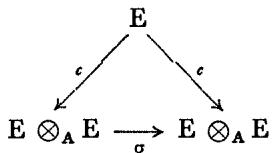
\includegraphics[keepaspectratio]{images/part004_07c99209.jpg}}

(其中 \(\sigma\) 是对称同态，使得 \(\sigma(x \otimes y) = y \otimes x\) ）是交换的（换句话说，只需余代数 E 与其反余代数（第1号，例2）相同即可）。

设 B 是交换 A-代数，u，v 是 C = Hom\_A(E, B) 的两个元素。

根据C中乘积的定义，uv和vu分别等于复合映射

\[
\mathrm{E} \xrightarrow {c} \mathrm{E} \otimes \mathrm{E} \xrightarrow {u \otimes v} \mathrm{B} \otimes \mathrm{B} \xrightarrow {m} \mathrm{B}
\]

和

\[
\mathrm{E} \xrightarrow {c} \mathrm{E} \otimes \mathrm{E} \xrightarrow {v \otimes u} \mathrm{B} \otimes \mathrm{B} \xrightarrow {m} \mathrm{B}.
\]

由此可知，若图(15)可交换，则代数 \(\operatorname{Hom}_{\mathbf{A}}(\mathbf{E}, \mathbf{B})\) 对每个可交换的A-代数B都是可交换的。为建立其逆命题，只需证明存在一个可交换的A-代数B以及两个A-线性映射 \(u, v\) 从 E 到 B 的映射，使得 \(m \circ (u \otimes v): \mathbf{E} \otimes \mathbf{E} \to \mathbf{B}\) 是单射。取 B 为代数 \(\mathsf{S}(\mathbf{E} \oplus \mathbf{E})\) ， \(u\) （相应地 \(v\) ）为典范映射 \(\mathbf{E} \oplus \mathbf{E} \to \mathsf{S}(\mathbf{E} \oplus \mathbf{E})\) 与映射 \(x \mapsto (x, 0)\) （相应地 \(x \mapsto (0, x)\) ）的复合，后者把 E 映入 \(\mathbf{E} \oplus \mathbf{E}\) 。若 \(h: \mathsf{S}(\mathbf{E}) \otimes \mathsf{S}(\mathbf{E}) \to \mathsf{S}(\mathbf{E} \otimes \mathbf{E})\) 是典范同构（ \(\S 6\) ，第6号，命题9）且 \(\lambda: \mathbf{E} \to \mathsf{S}(\mathbf{E})\) 是典范映射，那么 \(h^{-1} \circ m \circ (u \otimes v) = \lambda \otimes \lambda\) 。现在 \(\lambda \otimes \lambda\) 是单射的，因为 \(\lambda(\mathbf{E})\) 是 \(\mathsf{S}(\mathbf{E})\) 的直因子（II，§ 3，第7号，命题7的推论5）。

当余代数 E 满足命题2的条件时，称其为余交换的。

例子。（5）立即可以看出，余代数 A（第1号，例1）和余代数 \(\mathbf{A}^{(\mathbf{X})}\) （II，§ 11，第1号，例4）是余交换的。由第1号的公式（5）可知，余代数 S(M) 是余交换的。最后，对于 A-代数 B，使得 A-模 B 是投射的且有限生成的，要使余代数 \(\mathbf{B}^*\) （第1号，例3）是余交换的，其充分必要条件是 B 是交换的；因为（利用 A-模 B 与其双对偶的典范等同（II，§ 2，第7号）），这由图表（14）的交换性通过转置等价于表达 B 的交换性的图表（§ 1，第3号）这一事实得出。

命题3。设 E 是 A 上的一个余代数。为了使对于每个含单位元的 A-代数 B，A-代数 \(\operatorname{Hom}_{\mathbf{A}}(\mathbf{E},\mathbf{B})\) 是单位的，必要且充分条件是存在 E 上的一个线性形式 \(\gamma\) 使图表（16）交换

\begin{enumerate}
\def\labelenumi{(\arabic{enumi})}
\setcounter{enumi}{15}
\tightlist
\item
\end{enumerate}

\pandocbounded{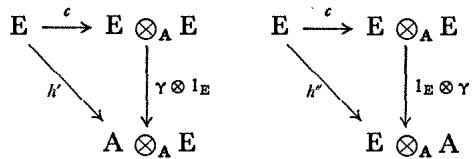
\includegraphics[keepaspectratio]{images/part004_cc0e83d1.jpg}}

（其中 \(c: \mathbf{E} \to \mathbf{E} \otimes_{\mathbf{A}} \mathbf{E}\) 是余积，并且 \(h'\) 和 \(h''\) 是典范同构（II，§ 3，第4号，命题4）。 \(\operatorname{Hom}_{\mathbf{A}}(\mathbf{E}, \mathbf{B})\) 的单位元则是线性映射 \(x \mapsto \gamma(x)1\) （其中1表示B的单位元）。

设 \(\gamma\) 是 E 上的一个线性形式，使得图表（16）交换。设 B 是带单位元 1 的含单位元 A-代数， \(\eta: \mathbf{A} \to \mathbf{B}\) 为典范映射， \(v = \eta \circ \gamma\) 为 A-代数 \(\mathbf{C} = \operatorname{Hom}_{\mathbf{A}}(\mathbf{E}, \mathbf{B})\) 的元素。对于每个元素 \(u \in \mathbf{C}\) ， \(uv\) 是复合映射

\[
\mathrm{E} \xrightarrow {c} \mathrm{E} \otimes \mathrm{E} \xrightarrow {1 _ {\mathrm{E}} \otimes \gamma} \mathrm{E} \otimes \mathrm{A} \xrightarrow {u \otimes \eta} \mathrm{B} \otimes \mathrm{B} \xrightarrow {m} \mathrm{B}.\tag{17}
\]

那么 \(uv = m \circ (u \otimes \eta) \circ h'' = u\) 。类似地可证明 \(vu = u\) ，因此 \(v\) 是 C 的单位元。反之，设 A-模 A ⊕ E 被赋予一个含单位元的代数结构，使得 \((a, x)(a', x') = (aa', ax' + a'x)\) （对 A 中的 \(a, a'\) 和 E 中的 \(x, x'\) ）。设 B 表示如此定义的 A-代数，并设 C 为 A-代数 Hom \(_A(E, B)\) 。假设 C 是含单位元的，并设 \(e: x \mapsto (\gamma(x), \lambda(x))\) 为其单位元（其中 \(\gamma(x) \in A\) 和 \(\lambda(x) \in E\) ）。另一方面，设 \(f\) 是 C 的元素 \(x \mapsto (0, x)\) 。直接计算表明 \(fe\) 是元素

\[
x \mapsto (0, (h ^ {\prime \prime}) ^ {- 1} ((1 _ {E} \otimes \gamma) (c (x))))
\]

此元素属于 C 。条件 \(fe = f\) 蕴含 (16) 中第二个图的交换性，并且类似地可看出条件 \(ef = f\) 蕴含 (16) 中第一个图的交换性。

E 上使图 (16) 交换的线性形式 \(\gamma\) 称为余代数 E 的余单位。一个余代数至多有一个余单位：因为它就是代数 \(\operatorname{Hom}_{\mathbf{A}}(\mathbf{E}, \mathbf{A})\) 的单位元。带有余单位的余代数称为余单位的。

例子。(6) 恒等映射是余代数 A 的余单位；在余代数 \(\mathbf{A}^{(\mathbf{X})}\) （第 1 号，例 4）上，线性形式 \(\gamma\) （使得 \(\gamma(e_x) = 1\) 对所有 \(x \in \mathbf{X}\) 成立）是余单位。在余代数 \(\mathbf{T}(\mathbf{M})\) （相应地 \(\mathbf{S}(\mathbf{M}), \bigwedge(\mathbf{M})\) ）上，线性形式 \(\gamma\) （满足 \(\gamma(1) = 1\) 且 \(\gamma(z) = 0\) ，其中 \(z\) 属于 \(\mathbf{T}^n(\mathbf{M})\) （相应地 \(\mathbf{S}^n(\mathbf{M}), \bigwedge^n(\mathbf{M})\) ）， \(n \geqslant 1\) ）是余单位。最后，设 B 是一个 A-代数，它是有限生成的投射 A-模，并且有单位元 \(e\) ；则在余代数 \(\mathbf{B}^*\) （第1号，例3）上，线性形式 \(\gamma: x^* \mapsto \langle e, x^* \rangle\) 是余单位，因为这个形式恰好是从 A 到 B 的 A-线性映射 \(\eta_e: \xi \mapsto \xi e\) 的转置，并且通过转置，图（16）的交换性可由那些表达（利用 \(\eta_e\) ）"\(e\) 是 B 的单位元"这一事实的图的交换性推出（ \(\S 1\) ，第 3 号）；同样的论证还表明，反之，若余代数 \(\mathbf{B}^*\) 具有一个余单位 \(\gamma\) ，则 \(\gamma\) 的转置定义 B 的单位元 \(e = {}^t\gamma(1)\) 。

命题 4. 设 E 是一个具有余单位 \(\gamma\) 的余代数，并假设 E 中存在一个元素 \(e\) ，使得 \(\gamma(e) = 1\) ；则 E 是子 A-模 Ae 与 \(\mathrm{E}_{\gamma} = \mathrm{Ker}(\gamma)\) 的直和，且

\[
c (e) \equiv e \otimes e (\mathrm{mod.} \mathrm{E} _ {\gamma} \otimes \mathrm{E} _ {\gamma})\tag{18}
\]

\[
\left\{c (x) \equiv x \otimes e + e \otimes x (\mathrm{mod.} \mathrm{E} _ {\gamma} \otimes \mathrm{E} _ {\gamma}) \quad \text { for all } x \in \mathrm{E} _ {\gamma}. \right.
\]

第一个断言是直接的，因为 \(\gamma(x - \gamma(x)e) = 0\) 以及关系 \(\gamma(\alpha e) = 0\) 蕴含 \(\alpha = 0\) 。设 \(c(e) = \sum_{i} s_i \otimes t_i\) ，使得

\[
e = \sum_ {i} \gamma (s _ {i}) t _ {i} = \sum_ {i} \gamma (t _ {i}) s _ {i}
\]

由 (16) 及 \(1 = \gamma(e) = \sum_{i} \gamma(s_i) \gamma(t_i)\) 得出。因此

\[
\begin{array}{r l} \sum_ {i} (s _ {i} - \gamma (s _ {i}) e) \otimes (t _ {i} - \gamma (t _ {i}) e) & = \sum_ {i} s _ {i} \otimes t _ {i} - \sum_ {i} e \otimes \gamma (s _ {i}) t _ {i} \\ & - \sum_ {i} \gamma (t _ {i}) s _ {i} \otimes e \\ & + \sum_ {i} \gamma (s _ {i}) e \otimes \gamma (t _ {i}) e \end{array}
\]

而根据上述关系，这正好是 \(c(e) - e \otimes e\) ；因此这证明了 (18) 中的第一个关系。另一方面，E \(\otimes\) E 作为直和的分解

\[
\mathbf {A} (e \otimes e) \oplus ((\mathbf {A} e) \otimes \mathbf {E} _ {\gamma}) \oplus (\mathbf {E} _ {\gamma} \otimes (\mathbf {A} e)) \oplus (\mathbf {E} _ {\gamma} \otimes \mathbf {E} _ {\gamma})
\]

使得我们可以写出，对于 \(x \in \mathbf{E}_{\gamma}\) , \(c(x) = \lambda(e \otimes e) + (e \otimes y) + (z \otimes e) + u\) （其中 \(u = \sum_{j} v_{j} \otimes w_{j}, y, z\) ，而 \(v_{j}\) 和 \(w_{j}\) 属于 \(\mathbf{E}_{\gamma}\) ）。余单位 \(\gamma\) 的定义随后给出 \(x = \lambda e + y = \lambda e + z\) ，并且由于 \(\gamma(x) = 0\) ，必然有 \(\lambda = 0, x = y = z\) ，由此得出 (18) 的第二个关系式。

注记。设 C 是一个有余单位的余结合 A-余代数，B 是一个含单位元的结合 A-代数，M 是一个左 B-模。A-双线性映射 \((b, m) \mapsto bm\) （从 \(B \times M\) 到 M 中）定义了一个 A-双线性映射

\[
\operatorname{Hom} _ {\mathbf {A}} (\mathrm{C}, \mathrm{B}) \times \operatorname{Hom} _ {\mathbf {A}} (\mathrm{C}, \mathrm{M}) \rightarrow \operatorname{Hom} _ {\mathbf {A}} (\mathrm{C}, \mathrm{M})
\]

这通过本号开头所述的一般程序完成。可以立即验证，该映射在 \(\operatorname{Hom}_{\mathbf{A}}(\mathbf{C}, \mathbf{M})\) 上定义了环 \(\operatorname{Hom}_{\mathbf{A}}(\mathbf{C}, \mathbf{B})\) 上的一个左模结构。

